\documentclass{article}
\usepackage[utf8]{inputenc}
\usepackage{subfig}
\usepackage{amsmath}

\usepackage{graphicx}
\usepackage[legalpaper, portrait, margin=0.5cm]{geometry}

\thispagestyle{empty}
% \renewcommand{\thesubfigure}{\roman{subfigure}}

\begin{document}

\begin{figure}[h]
        \centering
        \subfloat[analytical solution]{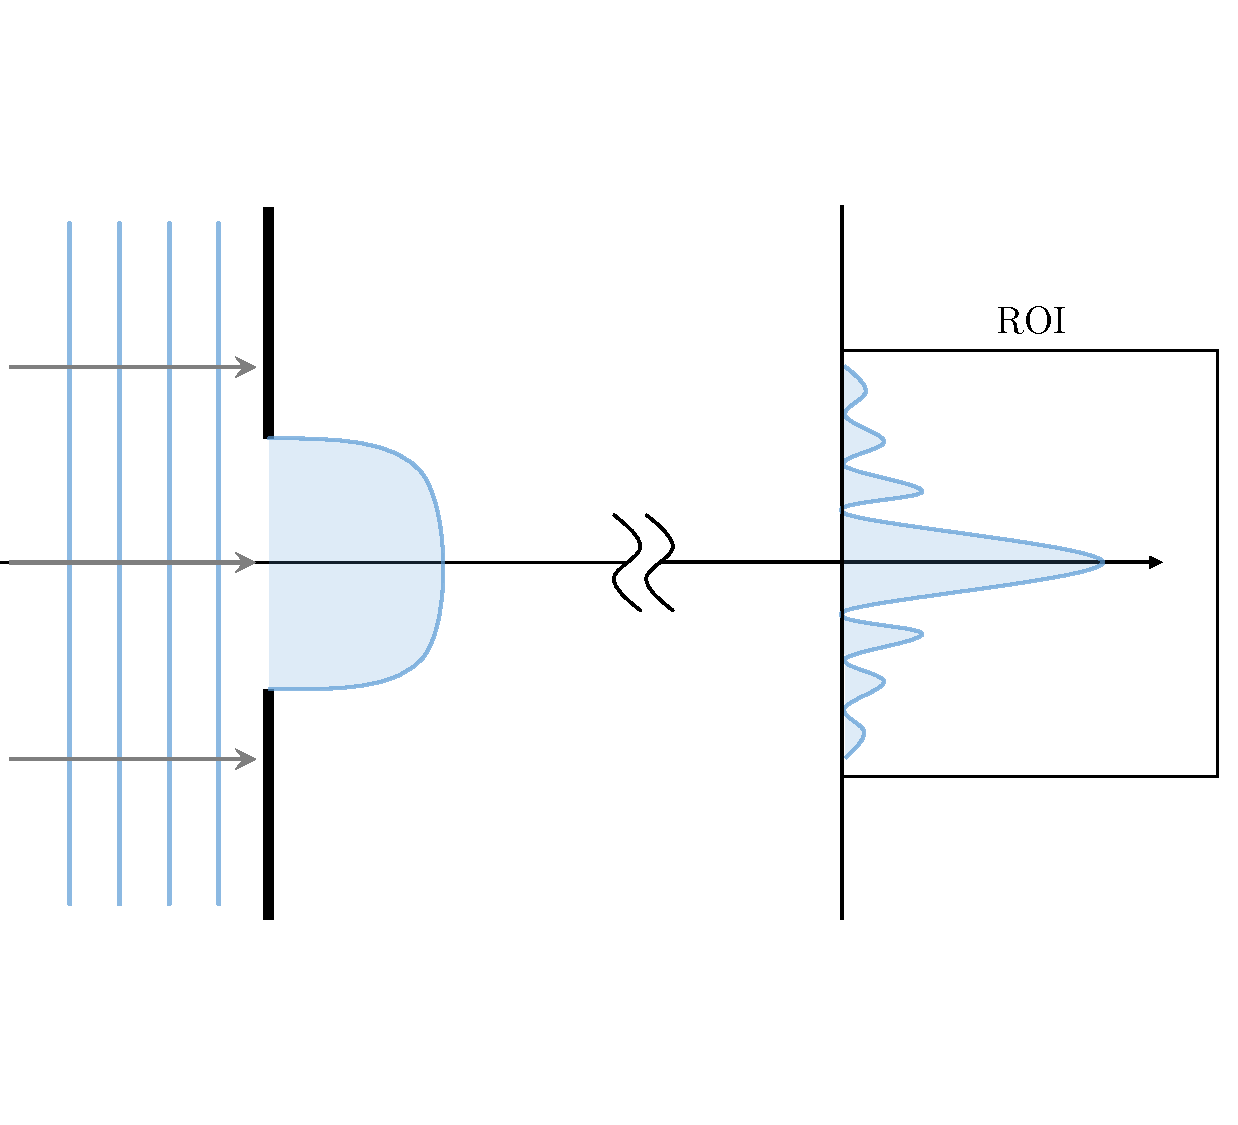
\includegraphics[width=6cm]{figures/ch02/replicas_aliasing_2.pdf}}\\
        \subfloat[]{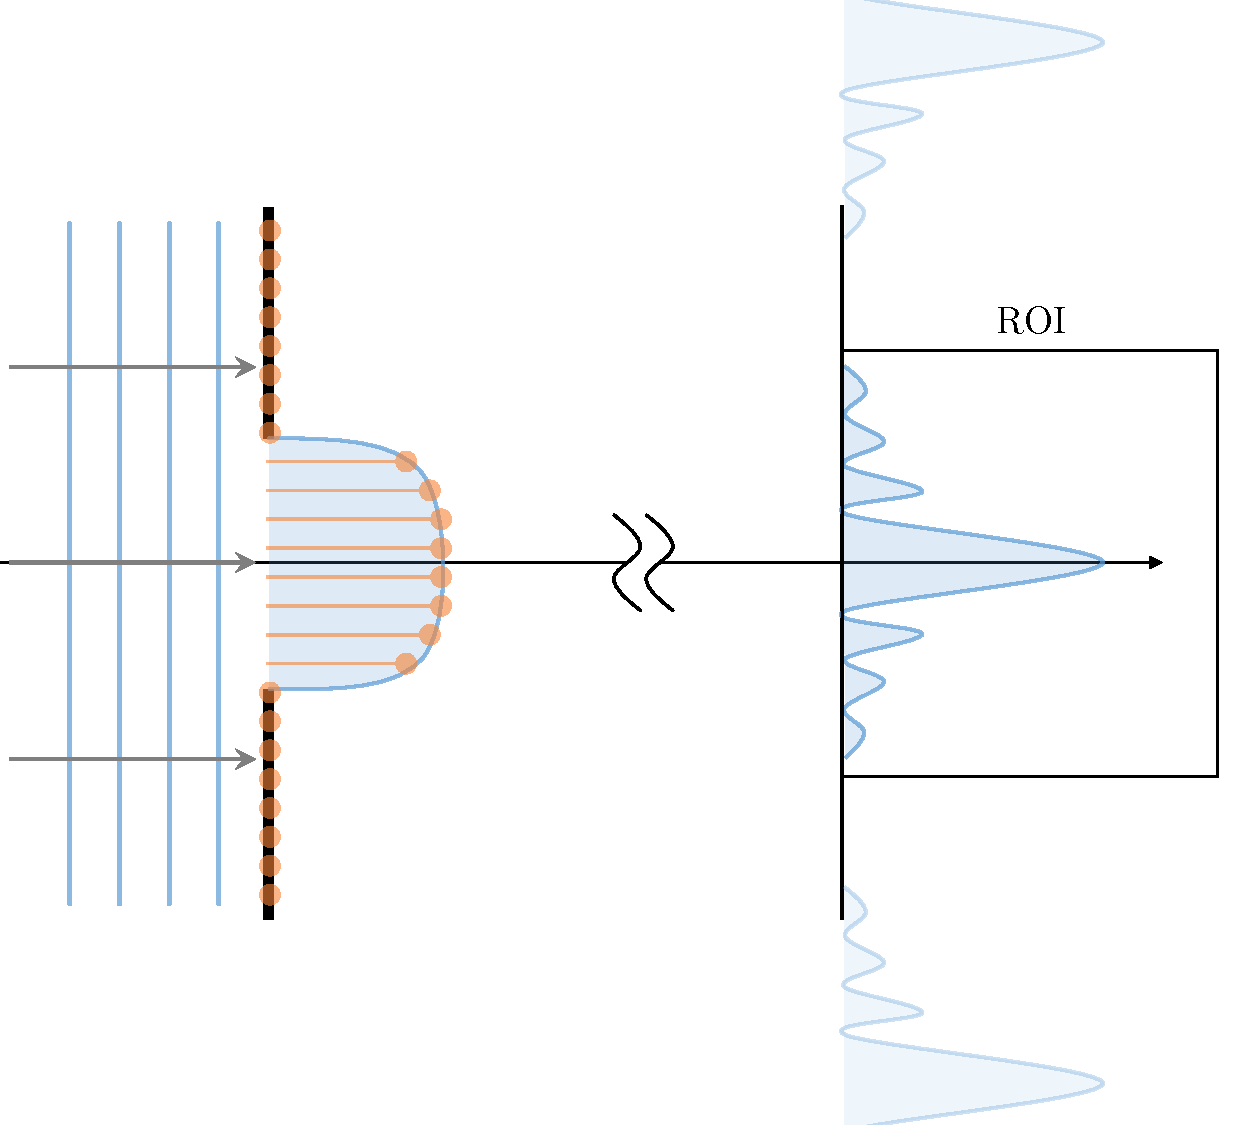
\includegraphics[width=6.cm]{figures/ch02/replicas_aliasing_3.pdf}}\hspace{0.5cm}
        \subfloat[]{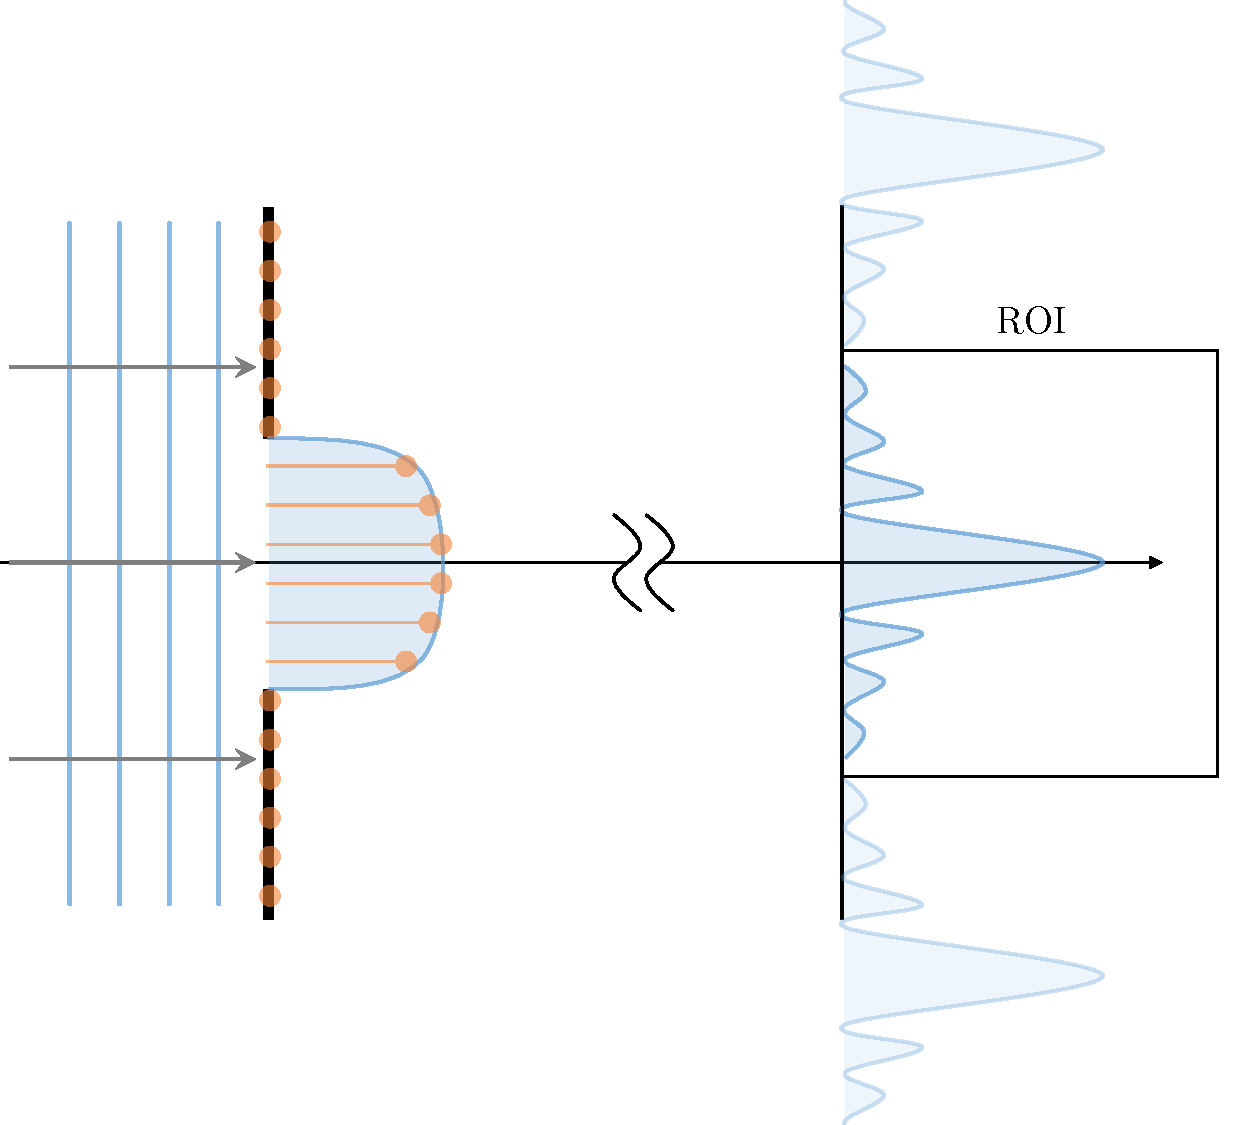
\includegraphics[width=6.cm]{figures/ch02/replicas_aliasing_4.pdf}}\hspace{0.5cm}
        \subfloat[]{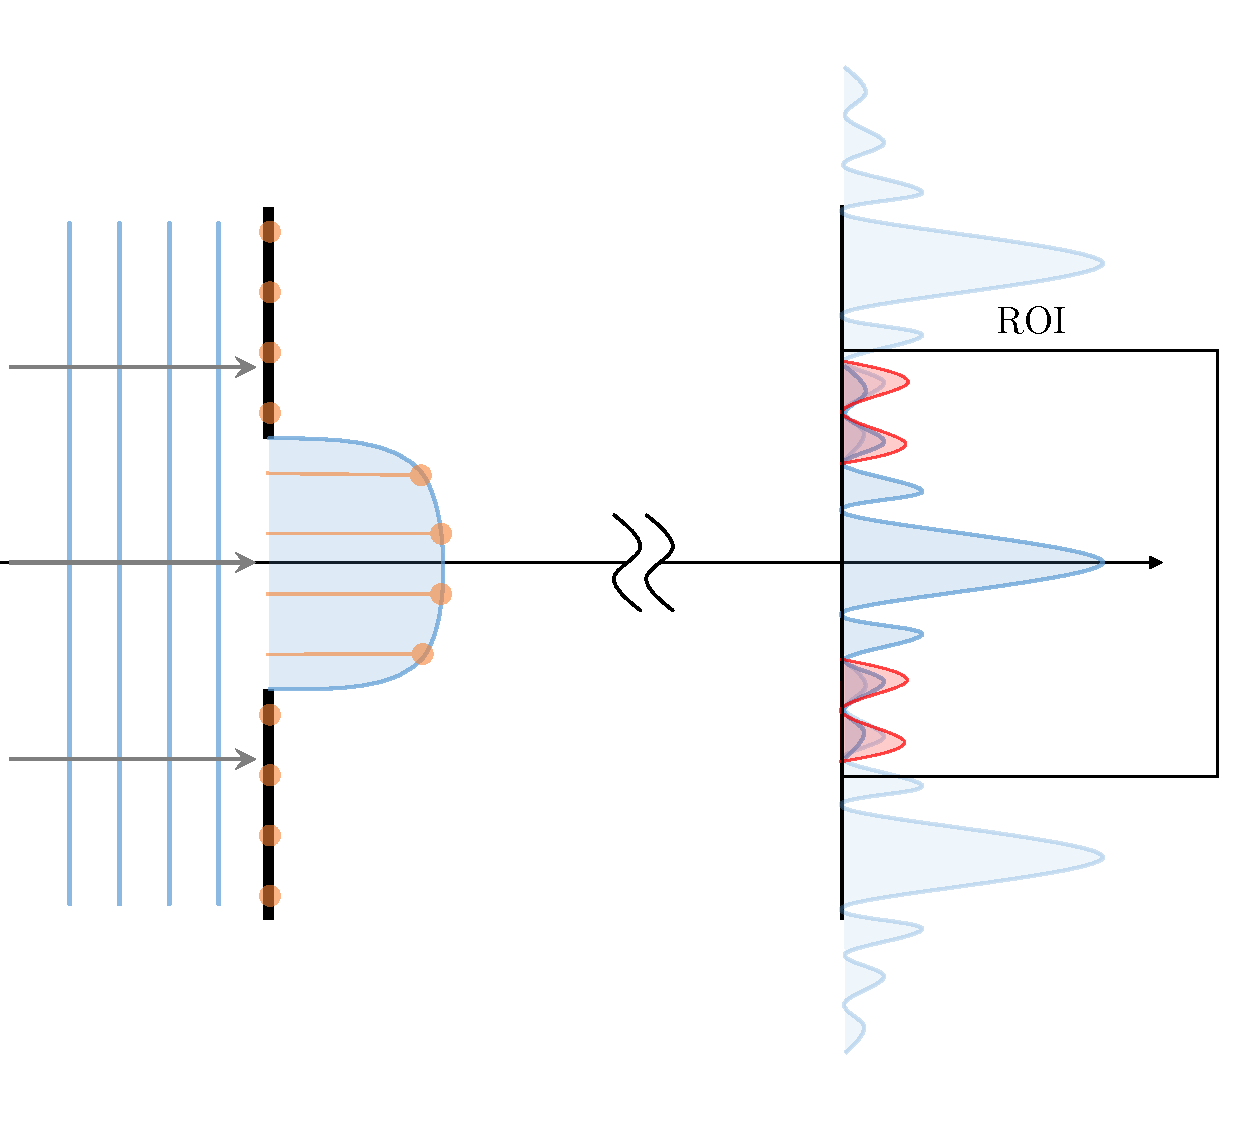
\includegraphics[width=6.cm]{figures/ch02/replicas_aliasing_5.pdf}}


\end{figure}


\end{document}